% See author's guidelines for Methods in Ecology and Evolution:
% http://www.methodsinecologyandevolution.org/view/0/authorGuidelines.html

\documentclass[12pt]{article}

% One-inch margins
\usepackage{fullpage}

% No orphans or widows
\usepackage[all]{nowidow}

% Additional math features
\usepackage{amsmath}

% Use mee bibliography style
\usepackage{natbib}
\bibliographystyle{mee}

% Include figures
\usepackage{graphicx}

% Definitions to make it easier to type
\newcommand{\MCMCMC}{(MC)$^{3}$}
\newcommand{\MCMCMCMC}{(MC)$^{4}$}

\begin{document}

% Double-spaced
\baselineskip 24pt

\begin{flushleft}

{\Large\textbf{Metropolis coupled Markov chain Monte Carlo
    for detecting rate shifts on phylogenetic trees}}

% Short title must be <= 45 characters (current: 47, including spaces)
\textbf{Short title:} Metropolis coupled MCMC for rate shift detection

% Recommended: 6000-7000 words, including tables, figure captions, references
\textbf{Word count:} 0

Carlos J. R. Anderson$^{1}$ and
Daniel L. Rabosky$^{1,*}$

$^{1}$Department of Ecology and Evolutionary Biology,
    University of Michigan, Ann Arbor, MI 48109, USA

$^{*}$Corresponding author: Daniel L. Rabosky (drabosky@umich.edu)

\end{flushleft}


\pagebreak[4]


% Maximum of 350 words
\section*{Abstract}

% Suppress indentation for the following paragraphs
{\setlength{\parindent}{0cm}

\textbf{1.}
BAMM (Bayesian Analysis of Macroevolutionary Mixtures) is a computer program
that uses Markov chain Monte Carlo (MCMC) to model complex dynamics
of speciation, extinction, and trait evolution on phylogenetic trees.
%
Previous versions of BAMM used a single Markov chain
to explore the landscape of models and their parameter values.
%
A single chain, however, may get stuck in local optima,
resulting in less mixing and more time needed for convergence.

\textbf{2.}
Here we describe an extension to BAMM
that implements Metropolis coupled MCMC [\MCMCMC].
%
In \MCMCMC, additional chains are introduced
that are able to explore more of the model landscape.
%
Swaps between chains may occur periodically,
so if a chain is stuck in a local optimum,
it may immediately jump to another area of the landscape.
%
In addition, we describe multi-core \MCMCMC,
which is able to run each chain on a separate CPU.

\textbf{3.}
We find that in both simulated data sets and an empirical data set,
\MCMCMC\ mixes better and reduces the time to convergence
compared to a single-chain MCMC.
%
Greater than four chains results in diminishing returns.

\textbf{4.}
\MCMCMC\ greatly improves the reliability of results in BAMM,
and we recommend its use in all future studies of macroevolutionary dynamics.
}

\begin{flushleft}
\textbf{Key-words:} BAMM, Bayesian, macroevolution, phylogeny, skink, speciation
\end{flushleft}


\pagebreak[4]


% State the reason for the work, the context and the hypotheses being tested
\section*{Introduction}

\subsection*{Background}

The variation in species richness and phenotypic diversity
we see today among groups of organisms is partly due
to the evolutionary processes of speciation and extinction.
%
Rates of speciation and extinction differ among groups
and have changed through time as a result of historical events,
such as environmental, phenotypic, and genetic changes.
%
For example, speciation could dramatically increase
during an adaptive radiation on a newly colonized island.
%
The phenotypic diversity of this colonizing group
could also increase as organisms evolve as they fill
the available ecological niches.


The processes of speciation and extinction with a group of organisms
have shaped the topology of their phylogenetic tree.
%
Phylogenetic trees can therefore be used to extract
information about the evolutionary processes that shaped them.
%
For example, an adaptive radiation could show up
as a burst in the number of splits and branches on a tree.
%
A phylogenetic tree would likely be composed of several processes,
each affecting the rate of diversification or morphological evolution
at a rate different from another such process.
%
A new method was developed recently to identify and characterize
such macroevolutionary processes across phylogenetic trees \citep{rab14plos}.


\subsection*{BAMM}

BAMM is a computer program that searches for models that best explain
complex dynamics of evolutionary processes on phylogenetic trees.
%
For speciation dynamics, a process is the rate of speciation
modeled as an exponential function through time.
%
A process may occur on any branch of a tree,
and all branches downstream of the process are under its influence.
%
There may be multiple processes on a single tree,
each process with its own set of parameters.
%
Processes may be nested, where a process within the clade
controlled by another process may occur.
%
In such a case, the process downstream of the ``ancestral'' process
takes over the dynamics of the branches downstream of it.


A BAMM model is a specific configuration of processes
(and their parameters) on a tree.
%
To search for plausible models that explain the observed tree,
BAMM uses reversible jump Markov Chain Monte Carlo (MCMC).
%
This method adds or removes processes on a tree,
moves processes from one location to another,
or changes specific parameter values within a process
in order to test the plausability of many models.
%
The advantage of using MCMC for model searching
is that BAMM does not produce a single best model,
but rather a set of models and their probability of explaining the data.


\subsection*{Metropolis coupled MCMC}

MCMC works by making changes, or ``moves,'' to the current model.
%
If the change improves the plausability of the new model,
this model becomes the current model (i.e., the move is accepted);
otherwise, the move is accepted with a probability
proportional to its plausability over the old model.
%
Previous versions of BAMM used a single Markov chain
to explore the landscape of models and their parameter values.
%
A single chain, however, may get stuck in local optima,
resulting in less mixing and more time needed for convergence.
%
Here we describe an extension to BAMM
that implements Metropolis coupled MCMC [\MCMCMC].
%
In \MCMCMC, additional chains are introduced
that are able to explore more of the model landscape.
%
Swaps between chains may occur periodically,
so if a chain is stuck in a local optimum,
it may immediately jump to another area of the landscape.
%
In addition, we describe multi-core \MCMCMC,
which is able to run each chain on a separate CPU.


% Include sufficient details for the work to be repeated
\section*{Materials and methods}

\subsection*{Metropolis coupled MCMC}

We followed \citet{alt04} for the implementation of \MCMCMC\ in BAMM.
%
For each Markov chain $i \in \{1, 2, \dots\}$, its temperature was set to
$\beta_i = [1 + \Delta T \times (i - 1)]^{-1}$,
where $\Delta T$ is the temperature increment parameter.
%
For example, if there are 4 chains and $\Delta T$ is 0.1,
the temperature of each chain is 1, 0.9091, 0.8333, and 0.7692.
%
The cold chain always has a temperature of 1.
%
The value of $\Delta T$ should be greater than 0
and chosen such that the probability of accepting a swap
is between 20\% and 60\% \citep{alt04}.


The temperature of chain $i$ goes into the calculation
of the acceptance probability $\alpha_i$ for a move proposal.
%
For moves that do not involve changes in the dimensionality of the model,
\[\alpha_i = \text{min}\left\{ 1,
    \left(
    \frac{f(\theta_i')}{f(\theta_i)} \times
    \frac{\pi(\theta_i')}{\pi(\theta_i)}
    \right)^{\beta_i} \times
    \frac{q(\theta_i | \theta_i')}{q(\theta_i' | \theta_i)}
\right\}\]
where $\theta_i$ and $\theta_i'$ are parameter vectors
corresponding to the current and proposed states for chain $i$,
$f$ and $\pi$ are the corresponding likelihood and prior density functions,
and $q(\theta_i' | \theta_i)$ is the relative probability
of proposing a move to parameter vector $\theta_i'$,
given that the current state is $\theta_i$.
%
A similar calculation was done for the acceptance probability for proposals
that change the dimensionality of the model.

After a certain number of generations, two randomly chosen chains $j$ and $k$
are swapped with acceptance probability
\[\alpha = \text{min}\left\{ 1,
    \left(\frac{f(\theta_k)}{f(\theta_j)}\right)^{\beta_j} \times
    \left(\frac{f(\theta_j)}{f(\theta_k)}\right)^{\beta_k}
\right\}\]


\subsection*{Implementation in BAMM}

In practice, the more Markov chains in the system,
the more calculations that must be performed,
and therefore the longer the program takes to run.
%
In a computer with multiple processors (``multi-core'')
each chain could run on a separate processor,
thereby reducing the actual time the program takes.
%
Because of differences among chain states as well as processor speeds,
chains will not all run at the same time.
%
A chain swap event, however, must occur between two chains
at the same generation.
%
Therefore, one must make sure that two chains that will swap
are ``synchronized.''


We implement such synchronization in BAMM
using a ``global exchange scheme'' \citep{alt04}.
%
In this scheme, chains run in parallel without synchronization
for a specific number of generations at which all chains must reach.
%
Once all chains reach this generation, a swap proposal occurs,
which may or may not be accepted.
%
The major disadvantage of this scheme
is that chains not involved in a swap
must still be synchronized with those chains in a swap,
possibly slowing down the run.
%
An advantage, however, is that this scheme is easy to implement.
%
When a swap is accepted, only the heat of the chains are swapped,
not their states, making it an efficient way of swapping.
%
The cold chain is that chain with the a temperature of 1.
%
We call this implementation
multi-core Metropolis coupled Markov Chain Monte Carlo [\MCMCMCMC].


\subsection*{Performance analysis}

We tested the performance of our implementation of \MCMCMC\ 
with both simulated trees and an empirical tree of Australian skinks.
%
Performance was assessed by comparing the effective size values
between runs without \MCMCMC\ and those with \MCMCMC.


For the simulated trees, we used 100 random trees generated by \citet{rab14plos}
under a pure-birth process at the root and four shifts
to diversity-dependent speciation-extinction processes.
%
We used BAMM (version 2.0.1) to model rates of species diversification
across each tree with and without \MCMCMC.
%
Runs with \MCMCMC\ were configured with four and eight chains,
the temperature increment parameter $\Delta T$ was set to 0.1,
and the swap period was set to 1,000 generations.
%
Runs went for 25 million generations,
sampling every 25,000 to produce a total of 1,000 samples.


As an emprical tree, we used the maximum clade credibility (MCC) tree
of Australian sphenomorphine skinks reconstructed by \citet{rab14sysbio}.
%
We used BAMM (version 2.0.0) to model rates of species diversification
across the tree with and without \MCMCMC.
%
We performed 25 runs with a single Markov chain [i.e., without \MCMCMC]
and 25 runs with four chains [i.e., with \MCMCMC].
%
The value of $\Delta T$ was set to 0.1
and the swap period was set to 1,000 generations.
%
Runs went for 100 million generations,
sampling every 100,000 to produce a total of 1,000 samples.
%
We assumed that the taxon sampling fraction was 85\%
of the extant species diversity.


% State the results, drawing attention to important details
% in tables and figures
\section*{Results}

For both the simulated trees and the empirical tree,
we found that with \MCMCMC\ runs had higher effective size
(Figure~\ref{fig:eff-size}).
%
For the simulated trees,
the mean effective size (and 95\% bootstrap confidence interval of the mean)
without \MCMCMC\ was 402 (331--459),
whereas with four and eight chains it was 548 (494--603) and 555 (494--611).
%
For the skink tree,
the mean effective size without \MCMCMC\ was 290 (205--380),
whereas with four chains it was 601 (558--644).

\begin{figure}
\begin{center}
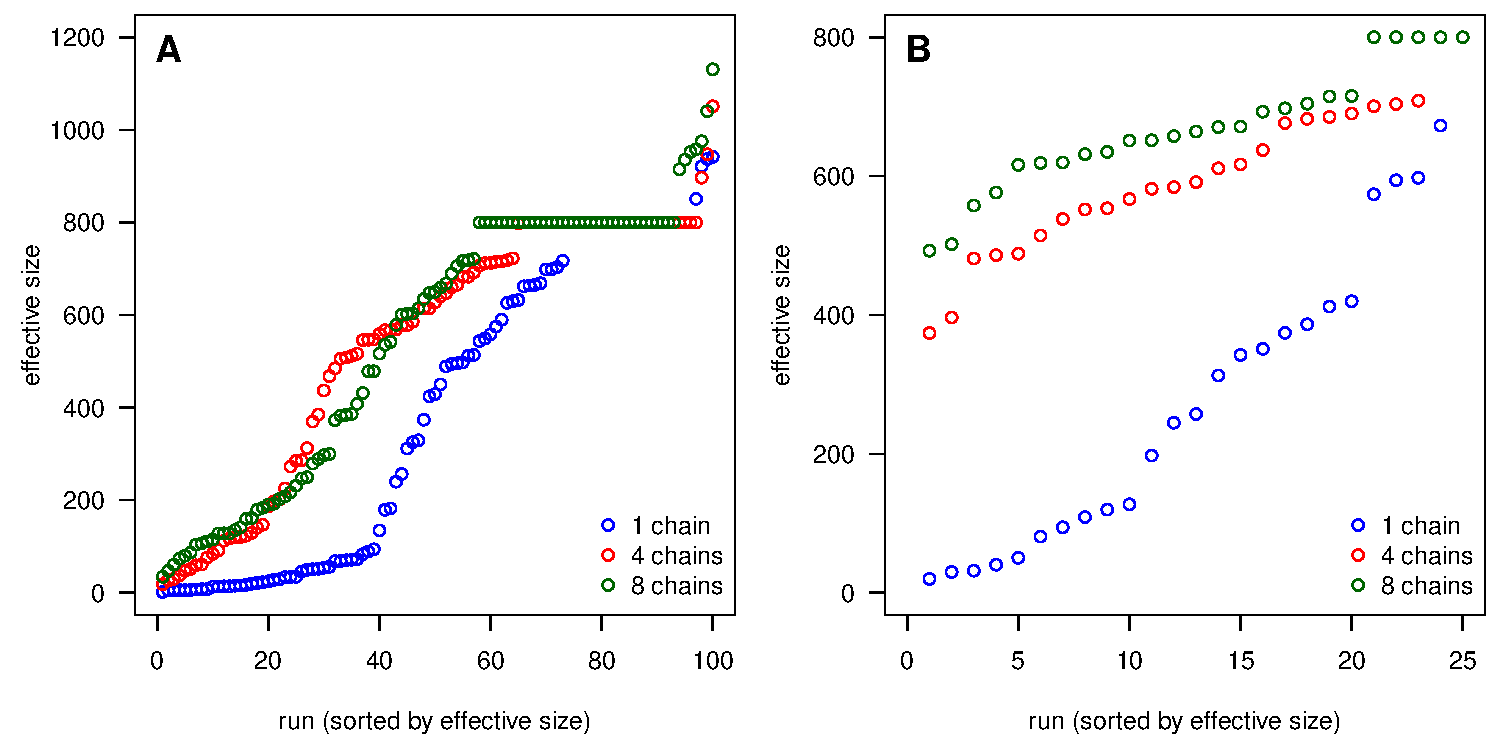
\includegraphics[width=14cm]{eff-size.pdf}
\end{center}
\caption{Effective sizes of the log-likelihood for
    (A) runs of 100 simulated trees and (B) 25 runs of the skink tree.
    Runs are sorted by their effective size.}
\label{fig:eff-size}
\end{figure}


For the simulated trees, which ran for 25 million generations,
the mean number of hours that runs took with
one chain, four chains, and eight chains were
6.3, 6.5, and 6.8 hr.
%
For the skink tree, which ran for 100 million generations,
the means were 18.8 hr for one chain,
and 20.7 hr for four chains.
%
The small difference in running times,
despite the difference in the number of chains,
was due to \MCMCMCMC, in which chains run in different processors.


% Point out the importance of the results and place them in the context
% of previous studies and in relation to the application of the work
% (expanding on the Synthesis and applications section of the Summary).
% Where appropriate, set out recommendations for management or policy
\section*{Discussion}

The discussion will go here.


\section*{Acknowledgements}

This research was supported in part through computational resources
and services provided by Advanced Research Computing
at the University of Michigan, Ann Arbor.


\bibliography{mc3}

\end{document}
